

\documentclass[journal]{IEEEtran}
%\documentclass[journal,12pt,onecolumn,draftclsnofoot,]{IEEEtran}

\usepackage{blindtext}
\usepackage{graphicx}
\usepackage{hyperref}
\usepackage{microtype}

\usepackage[cmex10]{amsmath}

\hyphenation{op-tical net-works semi-conduc-tor}
\begin{document}


% comment this out when you submit

\title{Duplicate Question Detection using Online Learning}
%\author{\IEEEauthorblockN{Author One\IEEEauthorrefmark{1},
%Author Two\IEEEauthorrefmark{2}, Author Three\IEEEauthorrefmark{3} and
%Author Four\IEEEauthorrefmark{4}}
%\IEEEauthorblockA{Department of Whatever,
%Whichever University\\
%Wherever\\
%Email: \IEEEauthorrefmark{1}author.one@add.on.net,
%\IEEEauthorrefmark{2}author.two@add.on.net,
%\IEEEauthorrefmark{3}author.three@add.on.net,
%\IEEEauthorrefmark{4}author.four@add.on.net}}

\author{\IEEEauthorblockN{Chapman Siu}
\IEEEauthorblockA{\\College of Computing, 
Georgia Institute of Technology\\
Atlanta, GA 30332-0280, USA\\
Email: chapmansiu@gatech.edu}}

\maketitle


\begin{abstract}
%\boldmath
An  integral  part  the learning  experiences for both on-campus and off-campus courses are  online  communities  such  as  Piazza.  Piazza is described as a ``Q\&A'' forum which is created for every class. An integral part of many online communities is the concept of ``voting'' to determine popular and useful information. However in many class orientated forums, this feature is not emphasised as post relevance tends to change relative to course assessments. Creating a way to understand quality posts can be beneficial for students and instructors, as it will reduce the clutter in the community by allow students to "see" important posts in the follow up section of different threads and for instructors to identify potential experts and teaching assistant candidates for future classes. 

In  this  project,  we  aim  to  develop  suitable  approach  for  understanding  quality  of  posts  through introducing  online  machine  learning  techniques  to  assist  with  reducing  clutter  within  young  online communities.


\end{abstract}

\begin{IEEEkeywords}
duplicate question, Piazza, online learning, machine learning
\end{IEEEkeywords}

\section{Introduction}

To understand and be able to explain quality posts, the type of modelling we are after is explanatory modelling, where we seek to provide causal explanations. One key consideration is that Shmueli\cite{modpred} describes how explanatory modelling does not always generalise well to predictive models. Shumueli\cite{modpred} also notes that the choice between explanatory and predictive modelling may affect the type of variables you use (variables have to make sense from a causal perspective), the type of preprocessing you may perform (data compression methods such as SVD may be inappropriate from a causal perspective), types of models you may build (ensemble of models would be inappropriate from a causal perspective). 

Comparing with previous studies, we are aiming to demonstrate how these techniques can be used in an online learning context. Online learning focuses on modelling data which arrives in sequential order to update our best predictor for future data as opposed to training on the whole training data set at once. This is important part of this project as with young communities, often the whole training data set will not be available until the community is relatively mature. This research would be similar to Zhang \emph{et al}\cite{dupred} conducted similar experiment with duplicate question detection via batch learning. Pal \emph{et al.}\cite{pal} explains that early identification and engagement with these users  can improve the experience of these users and more importantly improve the overall quality of participation within a community. Within Pal \emph{et al.}\cite{pal} retrospective analysis, it had already shown that some of the potential experts had already left the community when the analysis concluded leading to missed opportunities within the community. 



Furthermore to understand the type of questions which a community is asking can allow the noise to be diminished. For example on roughly 13 October 2016 the OMSCS admission results for Spring 2017 intake was annouced. Out of the newest 15 posts, 9 of them were new students questions or notes, with two threads having over 60 posts altogether. Similarly, reddit had 5 of 7 posts within the last 24 hours about new admissions, with 42 out of 44 comments in the respective posts in the threads on admissions.

Having adaptive duplication detection not only assists in special events but also in young communities, where there is a lack of training data or examples to create a sensible detection for duplicated questions. On forums like Piazza this would assist in reducing the amount of clutter which exists, similar to how stackoverflow closes duplicate questions for redundant questions to decrease the maintenance and people's resources on answering the same question\cite{dupred}. 

The following usage scenarios demonstrate the benefits of such a tool. 

\emph{Scenario} 1 - \emph{Without tool.} Steve recently gained admission to OMSCS program. However he is confused by the registration process and is unsure which course he should pick. He posts to the Google Plus community but received no response due to the flood of registration related posts. 

\emph{Scenario} 2 - \emph{With tool.} Steve recently gained admission to OMSCS program. However he is confused by the registration process and is unsure which course he should pick. He posts to the Google+ community. By using our automated tool, we can readily detect similar questions that have been asked before and direct Steve to a useful resource. 

We evaluate our approach on synthetically generated posts based on real questions asked on Google+ and Reddit, combined with unofficial FAQs generated by the community. We will also evaluate the performance by simulating a newly created Piazza forum to see if the tool has a similar efficacy. 

The main contributions of this paper are as follows.

\begin{itemize}
    \item We propose the problem of duplicate question detection in online communities. We procose a novel approach which considers and integrates multiple factors to detect duplicate questions.
    \item We evalute different types of communities based on real and synthetic questions.
\end{itemize}


The remainder of the paper is organised as follows. We elaborate on the motivation of our work and introduce online learning variants of Latent Dirichlet Allocation (LDA) and Word2Vec, and describe the other components of the overall framework. Next we will discuss some issues about the performance, efficiency and threats to validity. We will review related work, conclude the paper and mention future work. 


\section{Preliminaries}

%online Latent Dirichlet Allocation (online-LDA), which is used to extract topics from a young community in an iterative way and gain topic distribution from natural language description of questions.

%Online word2vec algorithm - word to vec is...

%\subsection{Motivation}

\subsection{Online Latent Dirichlet Allocation}

Online Latent Dirichlet Allocation is an online variant of Latent Dirichlet Allocation (LDA). LDA is a well-known topic modelling technique proposed by Blei \emph{et al.}\cite{lda}. LDA is a generative probabilistic model of a textual corpus (i.e., a set of textual documents), which takes a training textual corpus as input, and a number of parameters including the number of topics $(K)$ considered. In the training phase, for each document $s$, LDA will compute its topic distribution $\theta_s$, which is a vector with $K$ elements, and each element corresponds to a topic. The value of each element in $\theta_s$ is a real number from $0$ to $1$, which represents the proportion of the words in $s$ that belong to the corresponding topic in $s$. After training, LDA can be used to predict the topic distribution $\theta_m$ of a new document $m$. In our case, a document is the description of a question, and the topic is a higher level concept corresponding to a distribution of words. For example, we may have the topic ``admissions'', which is a distribution of words such as ``citizenship'', ``GRE'', ``TOEFL'', ``transcripts''. 

LDA can be extended in an online learning problem by reframing LDA using approximate inference techniques (variational inference) which then becomes an optimization problem and allows LDA to be trained via known approaches such as stochastic gradient descent\cite{onlinelda}. % explain this more...

% intuitively it means we find a problem which is easier to solve and show that it "converges in distribution" or close enough - according to KL divergence
% and based on this we can use gradient descent and by extension mini-batch+stochastic extensions. (left without proof?)




\subsection{Online Word2Vec}

Word2Vec is all about computing distributed vector representations of words. In this project we will be using the skip-gram variant. 

% from spark doco

The training objective of skip-gram is to learn word vector representations that are good at predicting its context in the same sentence. Mathematically, given a sequence of training words $w_1,w_2,...,w_T$, the objective of the skip-gram model is to maximize the average log-likelihood

$$ \frac{1}{T}\sum_{t=1}^T\sum_{j=-k}^{j=k} \log \Pr(w_{t+j} | w_t) $$

where $k$ is the size of the training window. 

In the skip-gram model, every word $w$ is associated with two vectors $u_w$ and $v_w$ which are vector representations of $w$ as word and context respectively. The probability of correctly predicting word $w_i$ given word $w_j$ is determined by the softmax model, which is

$$ \Pr (w_i | w_j) = \frac{\exp(u_{w_i}^T v_{w_j})}{\sum_{l=1}^V \exp(u_l^T v_{w_j}} $$

where $V$ is the vocabulary size. 

The skip-gram model with softmax is expensive because the cost of computing $\log (\Pr(w_i | w_j))$ is proportional to $V$, which can be easily in order of millions.% as stated in gensim negative sampling is used.- what does richard say about how negative sampling works?

% (see tensorflow, spark page) - can copy spark page for this.
% copy spark page
% http://spark.apache.org/docs/latest/mllib-feature-extraction.html#word2vec

Online variant of Word2Vec solves the online learning problem, by updating vocabulary whenever new documents are ingested. The new words are then initialized with random weights, whilst existing words retain their weights as normal. Then training will be again be initialised in an iterative fashion. % cite this?

\subsection{Online Latent Semantic Indexing}

Latent Semantic indexing is a transformation on bag-of-words models by applying truncated SVD to term-document matrices. This can be performed on word counts or tf-idf (term frequency-inverse document frequency). 

The online variant of latent semantic indexing is created through progressively updating the dictionary of words with a decay factor which will eventually ``forget'' older words. SVD truncation can be performed in an online fashion using known stochastic SVD algorithms. 

% expand this section.

\subsection{Matrix Cosine Similarity}

%(Write Why we don't need online learning here)

Cosine similarity is used to compute the similiarty between pairs of sets of words based on common words that they share. After preprocessing, the words are transformed into two bags (i.e. multisets) of words. For two sets of words $m$ and $n$, we represent the two bags of words that extracted as $Bag_m$ and $Bag_n$ respectively. Next we merge $Bag_m$ and $Bag_n$ and eliminate duplicate words to obtain the union set $Bag_u$, which contains $v$ words.  Following vector space modelling, we represent the two sentences as two vectors: $Vec_m = (wt_{m,1}, wt_{m, 2}, ..., wt_{m, v})$ and $Vec_n = (wt_{n,1}, wt_{n, 2}, ..., wt_{n, v})$. The weight $wt_{q, i}$  denotes the relative term frequency of the $i$-th word in sentence $q$'s title, which is computed as follows:

$$ wt_{q, i} = \frac{n_{q, i}}{\sum_v n_{q, v}} $$

where $n_{q, i}$ denotes the number of times the $i$-th word of $Bag_u$ appears in the sentence $q$, $\sum_v n_{q,v}$ denotes the total number of occurences of all words in the title of question $q$, where $v$ is the index of the word in $Bag_u$. We measure the similarity between two questions' titles by computing the cosine similarity of their vector representations $Vec_m$ and $Vec_n$ as follows:

$$ CosineSim(Vec_m, Vec_n) = \frac{\langle Vec_m,  Vec_n \rangle}{|Vec_m| | Vec_n| }$$

The numerator $\langle Vec_m , Vec_n \rangle$ which is the dot product of the two vectors 

$$ \langle Vec_m , Vec_n \rangle  = wt_{m, 1} \times wt_{n, 1} + ... + wt_{m, v} wt_{n, v} $$

The terms $|Vec_m|$ and $|Vec_n|$ in the denomiator denote the sizes of the two vectors respectively, where the size of $Vec_m$ is computed as 

$$ | Vec_m  | = \sqrt{wt_{m,1}^2 + wt_{m,2}^2 + ... + wt_{m,v}^2} $$

Cosine similarity measures do not require the whole corpus in order to compute similarity; rather it depends only on the pairwise sets of words. As such there is no online variant to cosine similarity as one does not need to build or store a corpus in its formulation.


\section{Proposed Approach}

In this section we will present the overall framework of duplicate question detection model. We will consider the components: title, tags, description, each having the three techniques applied. 

\subsection{Overall Framework}

% Insert some image of the framework and description of how it would work overtime. 

The framework of this prediction model using online learning consists of two phases: model building phase and prediction phase. In the model building phase, the goal is to train the models for building text features, which is then placed in a matrix similarity framework which become predictors for the supervised learning model. In the prediction phase the text models and the supervised models are used in conjunction to create a final prediction on similar questions.

The modelling process consists of three parts: 

\begin{itemize}
    \item Text Feature Building
    \item Matrix Cosine Similarity
    \item Model Training
\end{itemize}

On the prediction phase it involves three parts: 

\begin{itemize}
    \item Text Feature Prediction
    \item Matrix Cosine Similarity
    \item Model Prediction
\end{itemize}

%The framework relies on the existence of some questions which are known duplicates. This sample can be as small as 30 question pairs. 

\subsection{Text Feature Building}

To build text features, questions are to be collected in an iterative manner. Known pairs of similar questions are then to be labelled and preprocessed. In the preprocessing step, the title, description and tags (if applicable) are extracted. Next they are tokenized, common English stop words are removed and stemming is performed. Stop words are commonly occurring words, e.g., ``a'', ``the'', ``and''. Since they appear often, they possess low discriminatory power. Stemming is the process to reduce a word to its root. For exampling, using stemming on the words ``marks'', ``marking'', ``marked'' will result in the root word ``mark''. The Porter stemming algorithm from Python's gensim module was used. 

After these preprocessing step is performed, then each document have its text features using the three algorithms described in the previous section: Online Latent Dirichlet Allocation, Online Word2Vec, Online Latent Semantic Indexing. 

\subsection{Matrix Cosine Similarity}

Matrix Cosine Similiarity algorithm was described in the previous section. This technique is used on each of the word vector representations which were created in the text feature building phase in order to generate a similarity score. These scores will then be the features which are then passed into the supervised learning model. 

\subsection{Supervised Learning Models}

Now that modelling matrix created from the Matrix Cosine similarity step is created, we can simply pass it into any machine learning algorithm. In this paper, we used Random Forest to evaluate the effectiveness of our duplicate question detection model. 

\section{Experiments and Results}

\subsection{Experimental Setup}

Our online learning model is evaluated based on two different data sets. Firstly it is evaluated on historical questions in Stack Overflow. We parse data for `html' and `javascript' tags from January 2008 to October 2016 using Stackexchange API. We extract approximately 750 000 questions over 10 month period. The next dataset used is posts from OMSCS subreddit from October 2016 to November 2016 using Python's praw API. The similar questions were created by using FAQ datasets compiled by Reddit and Google+ OMSCS communities, and the similar questions were manually labelled. The experimental environment is from Windows 10 desktop machine, Intel i3 processor with 8GB of RAM. 

A Python library called Gensim was used to extract fields from the questions. Gensim is a flexible Python library statistical semantics. Gensim offered all the online text feature building capabilities within this setup. This includes stopword lists, Porter stemming, Online LDA, Online Latent Semantic Indexing, Online Word2Vec algorithms.

The Python library scikit-learn was used to perform supervised learning portion of the model. The two candidate models used were RandomForest and Logistic Regression. 

In Stack Overflow, users will manually detect duplicate questions. In our setup we successfully identified 7612 questions which were either marked as duplicates or manually linked to another question with tags ``html'' or ``javascript''. These questions formed the basis for our `similar questions' labels. 

For the OMSCS subreddit, we manually linked 30 posts with the relevant FAQ question, which is our corpus of known questions. 

Both of the two datasets were converted into a training and testing dataset as described in the table below. Since the training dataset is created through using similarity matrices, this means that a small number of linked/duplicated questions can yield a much larger training/testing set. 

\begin{table}[!t]
\centering
\caption{Statistics of the Training and the Test Set.}
 \begin{tabular}{l r r } 
 \hline
 Dataset & \#Similar Label & \#All \\ 
 \hline
 Training Stackoverflow & 1238 & 62499 \\ 
 %\hline
 Testing Stackoverflow & 258 & 10398  \\
 %\hline
 Training Reddit & 114 &   676 \\
 %\hline
 Testing Reddit & 23 & 139  \\
 \hline
\end{tabular}

\hfill \break

Note: \#Duplicate refers to the number of duplicate questions. \#All refers to the total number of questions.
\end{table}


\subsection{Evaluation Metrics}

To evaluate the performance, we will use recall-rate which is also used in \cite{dupred}. 

$$
\text{recall-rate} = \frac{N_\text{detected}}{N_\text{total}}
$$

This is a common metric which is used by \cite{dupred}.

\subsection{Research Questions and Findings}

Over a small subset and specific forums both of these appraoches appeared to perform reasonably well. 

However at the same time, even when a solution is reported as a match it can have some rather amusing answers. For example:




We are interested in answering the following research questions.

\subsubsection{How effective is our approach}


The recall rate for both datasets is shown below

\begin{table}[!t]
\centering
\caption{Recall rate for both datasets.}
 \begin{tabular}{l r } 
 \hline
 Dataset & Recall Rate  \\ 
 \hline
 Stackoverflow & 76.87\%  \\

 Reddit & 80.59\%  \\
 \hline
\end{tabular}


\end{table}

Our approach has seen fairly high recall rate, however if we were to productionize it and create a bot, it would have to follow the appraoch of Zhang \emph{et al}\cite{dupred}, where the top \emph{k} records are returned. This will ensure suitable answers are provided. 

For example, one unsuitable answer which appears in the community FAQs occur is telling users that ``We can not answer that for you here. We can, however, give you advice for the future.'' which has been linked to questions on topics like dealing with failing courses. Although the answer is suitable for the topic at hand, it is neither helpful and may be detrimental to the community. 


From a practical standpoint, this may not be that useful for the end user, as Reddit is more community orientated rather than a Q\&A discussion forum, which further increases the need for better answers compared with a Stack overflow setup. 

For example question answers below are two relatively common questions with the curated answer by the community. 

\begin{itemize}
    \item \emph{Will I get admitted?} We certainly can give you some feedback on this topic. However, we are not the admissions committee. We do not know exactly how decisions are made, so no one is liable here for your admissions status in the end.
    \item \emph{Why was I rejected?	} We can not answer that for you here. We can, however, give you advice for the future.
\end{itemize}

However in both instances the answer is not helpful for the end-user, and likely to be regarded as a low quality response. 



\subsubsection{What variables are important in our modelling routine, does it vary with different data sources}

The figures 1 and 2 demonstrate the variable importance metrics, it is clear that using different models will yield different parameter weightings. More importantly it reveals that LDA features appear to be the most significant. This also suggests that features which may incorporate information around the subject of the post may also improve performance. Recently including features like POS tags and named-entities have been used to great effect in information retrieval problems\cite{featurerich}.

\begin{figure}[ht]
\centering
\caption{Variable importance for the various text features for our Stack overflow model}
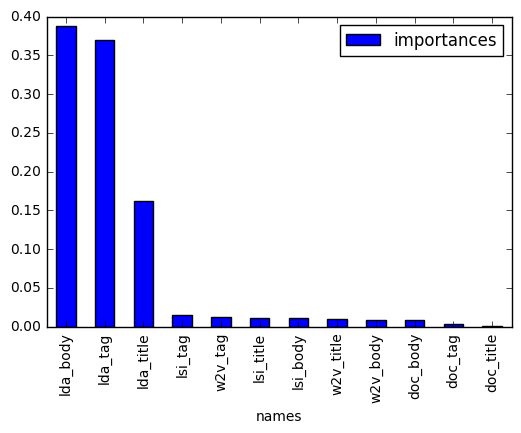
\includegraphics[width=0.4\textwidth]{so_varimp.png}
\end{figure}

\begin{figure}[ht]
\centering
\caption{Variable importance for the various text features for our Reddit model}
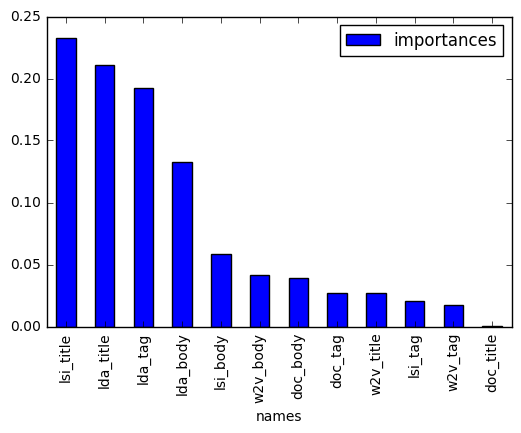
\includegraphics[width=0.4\textwidth]{reddit_varimp.png}
\end{figure}



\subsubsection{What is the effect of changing the types of models used}

When examining the different models, linear models and tree models were compared and contrasted. We achieved better results from using tree based models like random forest due to the interaction between the different features. Since different models have different parameters weights, having a tree-based model makes it easier to achieve reasonable results rather than needing to tune and fine the relevant interactions in the linear model framework as shown by Elith \emph{et al}\cite{gbminteraction}. 

\begin{table}[h!]
\centering
\caption{Recall rate for both datasets using different supervised models.}
 \begin{tabular}{l l r} 
 \hline
 Dataset & Model & Recall Rate  \\ 
 \hline
 Stackoverflow & Random Forest & 76.87\%  \\
 Stackoverflow & Logistic Regression & 37.12\%  \\
   Reddit & Random Forest & 80.59\%  \\
  Reddit & Logistic Regression & 10.84\%  \\
 \hline
\end{tabular}
\end{table}

\section{Discussion}

\subsection{Threats to Validity}

Threats include the ability of this approach to generalise to all young communities. As young communities is quite broad, the focus in this paper has been quite targeted, looking at computer science forums, and learning centers. The duplicate questions were also targeted and manually pruned. 

Threats to construct validity - suitability of evaluation metrics. In recent years ROUGE (Recall-Oriented Understudy for Gisting Evaluation)\cite{rouge} metric has been created for information retrieval problems, especially when reconstructing answers to be aligned with a human answer. These are based on the recall metric with noticeable improvements. In future iterations which focus more on how the answer is presented, would definitely focus on using this instead.



\section{Future Work}

As outlined in how this model was put together not all components are subject to online learning. More specifically the supervised portion used only batch learning techniques. Future work would examine using online supervised learning to augment this model as shown in Vowpal Wabbit\cite{vowpalwabbit}.

Within the Gensim library, the similarity matrix used was the cosine similarity. Chopra \emph{et al}\cite{simmatrix} has demonstrated that this measure of distance can be improved by learning different measures of similarity through utilizing weights within a Neural Network. 

Pal \emph{et al}\cite{pal} described how we can identify experts in MOOC communities, this notion of detecting experts early can be used to build a corpus of questions based on highly voted expert answers which can then be used to extend a simple Reddit bot in order to provide value to the community. 

% https://arxiv.org/pdf/1602.06023v5.pdf
Nallapati \emph{et al}\cite{featurerich} explains another way to extend word vectors to include linguistic features using technique they define as "Feature-rich Encoder". 

% insert some link to some paper
%Text summarization - longer texts means similarity breaks down really aggressively which can lead to better evaluation metrics such as ROGUE. 

\section{Conclusion}

In this paper we proposed a way to perform duplicate detection using online learning for Stack Overflow and Reddit. This approach measures similarity of two posts by comparing their observable factors, such as the titles, description and tags and their latent factors corresponding to the topic distribution that are learned from the natural language description of the question. Our approach also constructs other feature encodings including LSI and word2vec. 

We evaluated this approach using data available from Stack Overflow and Reddit which lead to experimental results of recall rates above 75\%.

In the future we plan to extend this approach with bleeding edge techniques such as feature rich-encoding to develop better techniques to improve the effectiveness of this approach.


% if have a single appendix:
%\appendix[Proof of the Zonklar Equations]
% or
%\appendix  % for no appendix heading
% do not use \section anymore after \appendix, only \section*
% is possibly needed

% use appendices with more than one appendix
% then use \section to start each appendix
% you must declare a \section before using any
% \subsection or using \label (\appendices by itself
% starts a section numbered zero.)
%


% use section* for acknowledgement

\begin{thebibliography}{1}

%\bibitem{IEEEhowto:kopka}
%H.~Kopka and P.~W. Daly, \emph{A Guide to \LaTeX}, 3rd~ed.\hskip 1em plus
%  0.5em minus 0.4em\relax Harlow, England: Addison-Wesley, 1999.
  
\bibitem{kincaid}
Kincaid, J. (2010, February 5). ``Piazzza gives classmates an online forum to trade their knowledge'''. Retrieved September 18, 2016, from \url{https://techcrunch.com/2010/02/05/piazzza-college-questions-answers/}

\bibitem{pal}
Pal, A., Farzan, R., Konstan, J. A., and Kraut, R. E. ``Early detection of potential experts in question answering communities.'' in \emph{User Modeling, Adaption and Personalization}. Springer, 2011, 231-242. Retrieved on 12 September 2016 from \url{http://researcher.ibm.com/researcher/files/us-apal/umap11_earlyexperts.pdf}

\bibitem{modpred}
Shmueli, G. (2010). ``To explain or to predict?'' \emph{Statistical Science} 25(3), 289–310. doi:10.1214/10-sts330. Retrieved on 30 September from \url{http://www.stat.berkeley.edu/~aldous/157/Papers/shmueli.pdf}

\bibitem{introIR}
Manning C.D., Raghavan P. and Schütze H. (2008), ``Introduction to Information Retrieval'', Cambridge University Press. 2008. Retreived on 30 September from \url{http://www-nlp.stanford.edu/IR-book/}

\bibitem{bog}
Bogatyy I. (2016) ``Predicting answer types for question-answering''. Retrieved on 30 September from \url{https://cs224d.stanford.edu/reports/Bogatyy.pdf}

\bibitem{dupred}
Zhang, Y., Lo, D., Xia, X., and Sun, J.-L. (2015). ``Multi-factor duplicate question detection in stack overflow'. \emph{Journal of Computer Science and Technology}, 30(5), 981–997. Retrieved on 17 September 2016 from \url{https://soarsmu.github.io/papers/jcst-duplicateqns.pdf}.  doi:10.1007/s11390-015-1576-4

\bibitem{lda}
Blei, D. M., Ng, A. Y. and Jordan, M. I. (2003). ``Latent dirichlet allocation''. J. Mach. Learn. Res., 3, 993--1022. doi: 10.1162/jmlr.2003.3.4-5.993. Retreived on 12 October from \url{www.jmlr.org/papers/volume3/blei03a/blei03a.pdf}

\bibitem{onlinelda}
Hoffman M. D., Blei D. M. and Bach F. (2010). ``Online Learning for Latent Dirichlet Allocation'' Retreived on 12 October from \url{http://www.cs.princeton.edu/~blei/papers/HoffmanBleiBach2010b.pdf}

\bibitem{simmatrix}
Chopra S., Hadsell, R. and LeCun, Y. (2005). ``Learning a Similarity Metric Discriminatively, with Application to Face
Verification'' Retreived on 17 November from \url{http://yann.lecun.com/exdb/publis/pdf/chopra-05.pdf}

\bibitem{featurerich}
Nallapati R., Zhou B., Noueira dos santos C., Gulcehre C. and Xiang B. (2016). ``Abstractive Text Summarization Using Sequence-to-Sequence RNNs and Beyond'' Retreived on 23 November from \url{https://arxiv.org/abs/1602.06023}

\bibitem{gbminteraction}
Elith J. and Leathwick J. (2016). ``Boosted Regression Trees for ecological modelling'' Retreived on 24 November from \url{https://cran.r-project.org/web/packages/dismo/vignettes/brt.pdf}



\bibitem{vowpalwabbit}
Agarwal A., Chapelle O., Dudik M. and Langford J. (2012). ``A Reliable Effective Terascale Linear Learning System''. In Journal of Machine Learning Research 2012. Retreived on 24 November from \url{https://arxiv.org/pdf/1110.4198v3.pdf}


\bibitem{rouge}
Lin CY. (2004). ``ROUGE: A Package for Automatic Evaluation of Summaries''. In Proceedings of the Workshop on Text Summarization Branches Out (WAS 2004), Barcelona, Spain, July 25 - 26, 2004. Retreived on 24 November from \url{http://www.aclweb.org/anthology/W/W04/W04-1013.pdf}

\end{thebibliography}

% biography section
% 
% If you have an EPS/PDF photo (graphicx package needed) extra braces are
% needed around the contents of the optional argument to biography to prevent
% the LaTeX parser from getting confused when it sees the complicated
% \includegraphics command within an optional argument. (You could create
% your own custom macro containing the \includegraphics command to make things
% simpler here.)
%\begin{biography}[{\includegraphics[width=1in,height=1.25in,clip,keepaspectratio]{mshell}}]{Michael Shell}
% or if you just want to reserve a space for a photo:

\begin{IEEEbiography}[{
\includegraphics[width=1in,height=1.25in,clip,keepaspectratio]{picture}}]{Chapman Siu}
is a Masters candidate from Georgia Institute of Technology. Chapman is also a lion.
\end{IEEEbiography}

% You can push biographies down or up by placing
% a \vfill before or after them. The appropriate
% use of \vfill depends on what kind of text is
% on the last page and whether or not the columns
% are being equalized.

%\vfill

% Can be used to pull up biographies so that the bottom of the last one
% is flush with the other column.
%\enlargethispage{-5in}

% comment this out when you submit

% that's all folks
\end{document}


